% !TEX program = xelatex
% 使用 UTF-8 编码
\documentclass[UTF8]{ctexart}

% --- 全局宏包与设置 (所有设置都在这里) ---
\usepackage{geometry}
\geometry{a4paper, left=2.5cm, right=2.5cm, top=2.5cm, bottom=2.5cm} % 正文页边距

\usepackage{graphicx}  % 用于插入图片
\usepackage{amsmath}   % 用于数学公式
\usepackage{listings}  % 用于插入代码
\usepackage{xcolor}    % 用于定义颜色
\usepackage{hyperref}  % 用于生成超链接
\usepackage{placeins}  %用于控制图片位置
% --- 字体设置 ---
% 确保你的系统已经安装了这些字体
\setmainfont{Times New Roman} % 英文和数字字体
\setCJKmainfont{SimSun} % 中文字体 (宋体)

% --- 超链接设置 ---
\hypersetup{
    colorlinks=true,
    linkcolor=blue,
    filecolor=magenta,
    urlcolor=cyan,
}

% --- 代码块样式定义 ---
\definecolor{codegreen}{rgb}{0,0.6,0}
\definecolor{codegray}{rgb}{0.5,0.5,0.5}
\definecolor{codepurple}{rgb}{0.58,0,0.82}
\definecolor{backcolour}{rgb}{0.95,0.95,0.92}
\lstdefinestyle{mystyle}{
    backgroundcolor=\color{backcolour},
    commentstyle=\color{codegreen},
    keywordstyle=\color{magenta},
    numberstyle=\tiny\color{codegray},
    stringstyle=\color{codepurple},
    basicstyle=\ttfamily\footnotesize,
    breakatwhitespace=false,
    breaklines=true,
    captionpos=b,
    keepspaces=true,
    numbers=left,
    numbersep=5pt,
    showspaces=false,
    showstringspaces=false,
    showtabs=false,
    tabsize=2
}
\lstset{style=mystyle}


% --- 文档开始 ---
\begin{document}

% 插入封面
% !TEX program = xelatex
% 这是中国海洋大学本科毕业论文的封面模板
% 请在主文档中使用 % !TEX program = xelatex
% 这是中国海洋大学本科毕业论文的封面模板
% 请在主文档中使用 % !TEX program = xelatex
% 这是中国海洋大学本科毕业论文的封面模板
% 请在主文档中使用 \input{titlepage.tex} 调用此文件

\thispagestyle{empty} % 封面不显示页码


% --- 自定义命令 ---
\newcommand{\degreeclass}{本科} % 学位类型
\newcommand{\universityname}{中国海洋大学}

% --- 封面内容 ---
\begin{titlepage}
    \centering

    % 页眉信息
    \vspace*{-2cm} % 调整与页面顶部的距离
    \vspace{1.5cm} % 与Logo之间的垂直间距

    % Logo
    \begin{flushright}
        \includegraphics[width=0.15\textwidth]{pic/ouc_logo.eps} % 请确保 OUC_Logo.png 文件存在且路径正确
    \end{flushright}
    \vspace{2cm} % 与正标题之间的垂直间距

    % 主标题
    {\zihao{2} \heiti \textbf{系统开发工具基础实验报告}}
    \par \vspace{1.5cm} % 与副标题之间的垂直间距

    % 副标题 (题目)
    {\zihao{2} \heiti \textbf{题目:}\quad \underline{版本控制(git)}}
    \par \vspace{3cm} % 与学生信息之间的垂直间距

    % 学生及指导教师信息
    \begin{tabular}{r l}
        \zihao{-4} \songti 学生姓名\quad & \underline{周洋迅} \quad 学号\quad \underline{24020007175} \\
        \zihao{-4} \songti 学部、学院(中心)\quad & \underline{信息科学与工程学部} \\
        \zihao{-4} \songti 专业\quad & \underline{计算机科学与技术} \\
        \zihao{-4} \songti 日期\quad & \underline{2025} 年 \underline{8} 月 \underline{29} 日 \\
        \zihao{-4} \songti github链接\quad & \underline{https://github.com/zysgusg/SysDevelopmentTools}\\
    \end{tabular}
    \par \vspace{2cm} % 与学校名称之间的垂直间距

    % 学校名称
    {\zihao{3} \heiti \textbf{\universityname}}
    \par \vspace{1cm} % 页面底部留白

\end{titlepage} 调用此文件

\thispagestyle{empty} % 封面不显示页码


% --- 自定义命令 ---
\newcommand{\degreeclass}{本科} % 学位类型
\newcommand{\universityname}{中国海洋大学}

% --- 封面内容 ---
\begin{titlepage}
    \centering

    % 页眉信息
    \vspace*{-2cm} % 调整与页面顶部的距离
    \vspace{1.5cm} % 与Logo之间的垂直间距

    % Logo
    \begin{flushright}
        \includegraphics[width=0.15\textwidth]{pic/ouc_logo.eps} % 请确保 OUC_Logo.png 文件存在且路径正确
    \end{flushright}
    \vspace{2cm} % 与正标题之间的垂直间距

    % 主标题
    {\zihao{2} \heiti \textbf{系统开发工具基础实验报告}}
    \par \vspace{1.5cm} % 与副标题之间的垂直间距

    % 副标题 (题目)
    {\zihao{2} \heiti \textbf{题目:}\quad \underline{版本控制(git)}}
    \par \vspace{3cm} % 与学生信息之间的垂直间距

    % 学生及指导教师信息
    \begin{tabular}{r l}
        \zihao{-4} \songti 学生姓名\quad & \underline{周洋迅} \quad 学号\quad \underline{24020007175} \\
        \zihao{-4} \songti 学部、学院(中心)\quad & \underline{信息科学与工程学部} \\
        \zihao{-4} \songti 专业\quad & \underline{计算机科学与技术} \\
        \zihao{-4} \songti 日期\quad & \underline{2025} 年 \underline{8} 月 \underline{29} 日 \\
        \zihao{-4} \songti github链接\quad & \underline{https://github.com/zysgusg/SysDevelopmentTools}\\
    \end{tabular}
    \par \vspace{2cm} % 与学校名称之间的垂直间距

    % 学校名称
    {\zihao{3} \heiti \textbf{\universityname}}
    \par \vspace{1cm} % 页面底部留白

\end{titlepage} 调用此文件

\thispagestyle{empty} % 封面不显示页码


% --- 自定义命令 ---
\newcommand{\degreeclass}{本科} % 学位类型
\newcommand{\universityname}{中国海洋大学}

% --- 封面内容 ---
\begin{titlepage}
    \centering

    % 页眉信息
    \vspace*{-2cm} % 调整与页面顶部的距离
    \vspace{1.5cm} % 与Logo之间的垂直间距

    % Logo
    \begin{flushright}
        \includegraphics[width=0.15\textwidth]{pic/ouc_logo.eps} % 请确保 OUC_Logo.png 文件存在且路径正确
    \end{flushright}
    \vspace{2cm} % 与正标题之间的垂直间距

    % 主标题
    {\zihao{2} \heiti \textbf{系统开发工具基础实验报告}}
    \par \vspace{1.5cm} % 与副标题之间的垂直间距

    % 副标题 (题目)
    {\zihao{2} \heiti \textbf{题目:}\quad \underline{版本控制(git)}}
    \par \vspace{3cm} % 与学生信息之间的垂直间距

    % 学生及指导教师信息
    \begin{tabular}{r l}
        \zihao{-4} \songti 学生姓名\quad & \underline{周洋迅} \quad 学号\quad \underline{24020007175} \\
        \zihao{-4} \songti 学部、学院(中心)\quad & \underline{信息科学与工程学部} \\
        \zihao{-4} \songti 专业\quad & \underline{计算机科学与技术} \\
        \zihao{-4} \songti 日期\quad & \underline{2025} 年 \underline{8} 月 \underline{29} 日 \\
        \zihao{-4} \songti github链接\quad & \underline{https://github.com/zysgusg/SysDevelopmentTools}\\
    \end{tabular}
    \par \vspace{2cm} % 与学校名称之间的垂直间距

    % 学校名称
    {\zihao{3} \heiti \textbf{\universityname}}
    \par \vspace{1cm} % 页面底部留白

\end{titlepage}

\newpage
\tableofcontents % 自动生成目录
\newpage

% --- 实验内容 ---
\section{练习内容}
\begin{enumerate}
		\subsection{基础}
		\item git help <command>: 获取 git 命令的帮助信息
        \item git init: 创建一个新的 git 仓库,其数据会存放在一个名为 .git 的目录下
        \item git status:显示当前的仓库状态
        \item git add <filename>: 添加文件到暂存区
        \item git commit: 创建一个新的提交
        \item git log: 显示历史日志
        \item git diff <filename>: 显示与暂存区文件的差异
        \item git checkout <revision>: 更新 HEAD(如果是检出分支则同时更新当前分支)
    
    \subsection{合并与分支}
        \item git branch: 显示分支
        \item git branch <name>: 创建分支
        \item git checkout -b <name>: 创建分支并切换到该分支;相当于 git branch <name>; git checkout <name>
        \item git merge <revision>: 合并到当前分支

    \subsection{远端操作}
        \item git remote: 列出远端
        \item git remote add <name> <url>: 添加一个远端
        \item git push <remote> <local branch>:<remote branch>: 将对象传送至远端并更新远端引用
        \item git branch --set-upstream-to=<remote>/<remote branch>: 创建本地和远端分支的关联关系
        \item git fetch: 从远端获取对象/索引
        \item git pull: 相当于 git fetch; git merge
        \item git clone: 从远端下载仓库
    
    \subsection{撤销}  
        \item git commit --amend: 编辑提交的内容或信息
        \item git reset HEAD <file>: 恢复暂存的文件
        \item git checkout -- <file>: 丢弃修改
        
\end{enumerate}


% --- 实验结果 ---
\section{练习结果}
\subsection{结果截图}
\begin{figure}[htbp] % h: here, t: top, b: bottom, p: page of floats
    \centering
    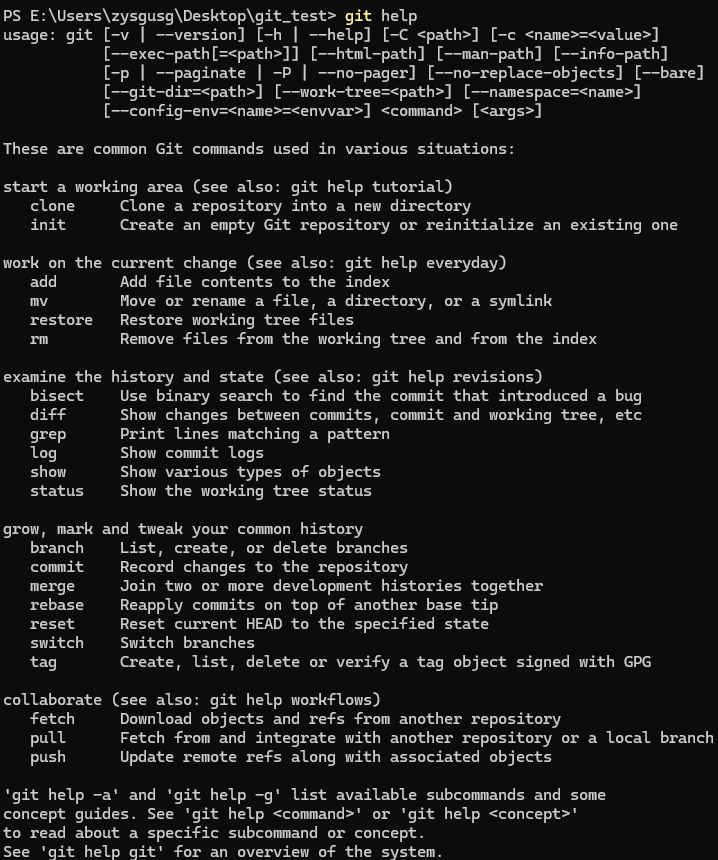
\includegraphics[width=0.8\textwidth]{1.png} 
    \caption{git help}
\end{figure}
\begin{figure}[htbp]
    \centering
    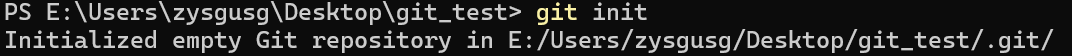
\includegraphics[width=0.8\textwidth]{2.png} 
    \caption{git init}
\end{figure}
\begin{figure}[htbp]
    \centering
    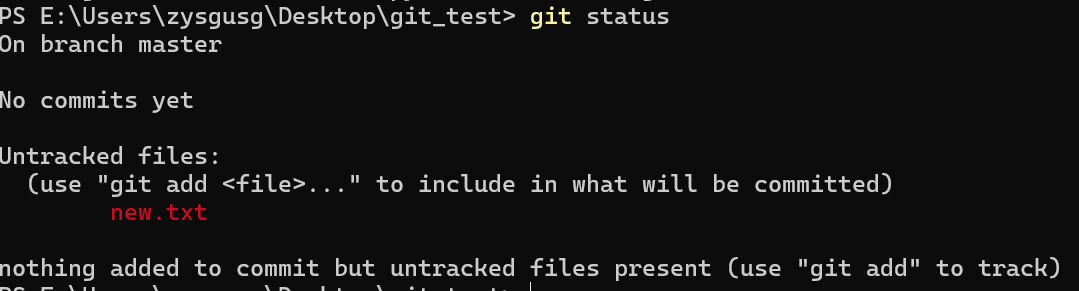
\includegraphics[width=0.8\textwidth]{3.png} 
    \caption{git status}
\end{figure}
\begin{figure}[htbp]
    \centering
    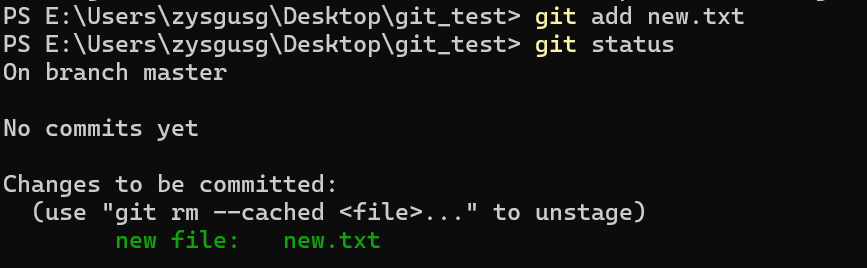
\includegraphics[width=0.8\textwidth]{4.png} 
    \caption{git add}
\end{figure}
\begin{figure}[htbp]
    \centering
    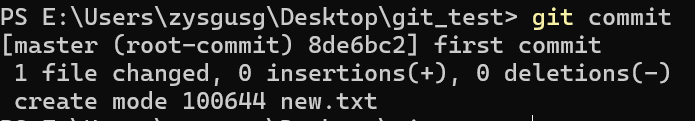
\includegraphics[width=0.8\textwidth]{5.png} 
    \caption{git commit}
\end{figure}
\begin{figure}[htbp]
    \centering
    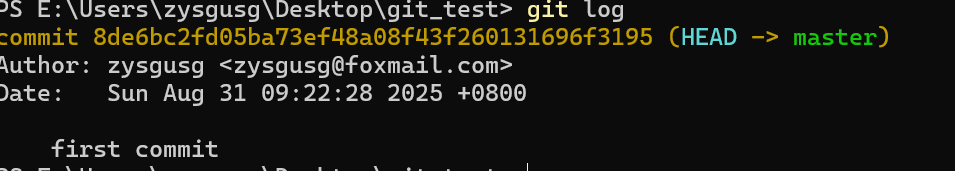
\includegraphics[width=0.8\textwidth]{6.png} 
    \caption{git log}
\end{figure}
\begin{figure}[htbp]
    \centering
    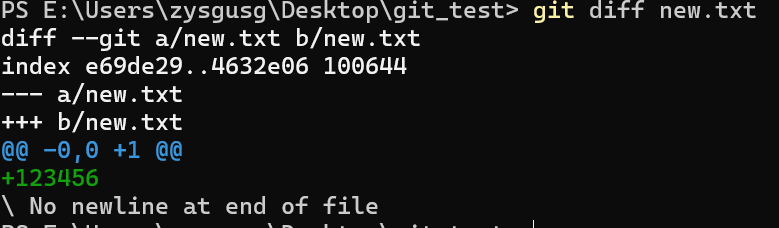
\includegraphics[width=0.8\textwidth]{7.png} 
    \caption{git diff <filename>}
\end{figure}
\begin{figure}[htbp]
    \centering
    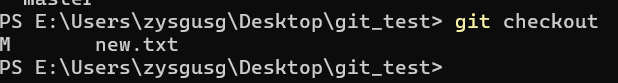
\includegraphics[width=0.8\textwidth]{8.png} 
    \caption{git checkout <revision>}
\end{figure}
\begin{figure}[htbp]
    \centering
    
\includegraphics[width=0.8\textwidth]{9.png} 
    \caption{git branch}
\end{figure}
\begin{figure}[htbp]
    \centering
    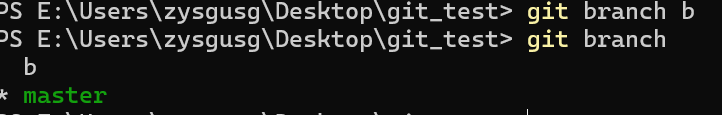
\includegraphics[width=0.8\textwidth]{10.png} 
    \caption{git branch <name>}
\end{figure}
\begin{figure}[htbp]
    \centering
    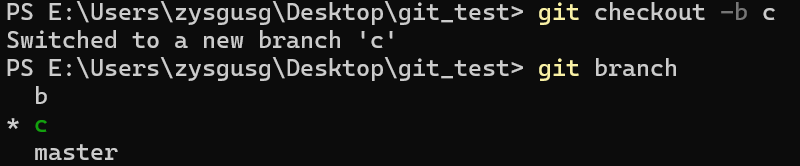
\includegraphics[width=0.8\textwidth]{11.png} 
    \caption{git checkout -b <name>}
\end{figure}
\begin{figure}[htbp]
    \centering
    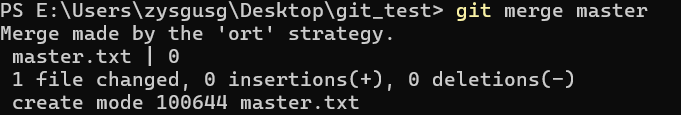
\includegraphics[width=0.8\textwidth]{12.png} 
    \caption{git merge <revision>}
\end{figure}
\begin{figure}[htbp]
    \centering
    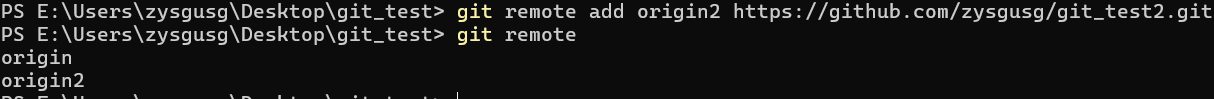
\includegraphics[width=0.8\textwidth]{13.png} 
    \caption{git remote}
\end{figure}
\begin{figure}[htbp]
    \centering
    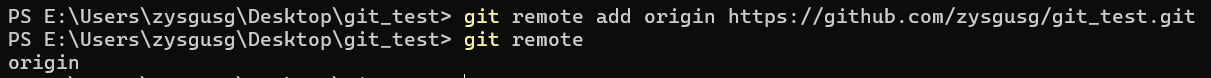
\includegraphics[width=0.8\textwidth]{14.png} 
    \caption{{git remote add <name> <url>}}
\end{figure}
\begin{figure}[htbp]
    \centering
    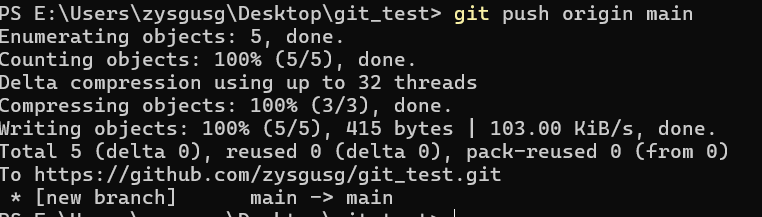
\includegraphics[width=0.8\textwidth]{15.png} 
    \caption{git push <remote> <local branch>:<remote branch>}
\end{figure}
\begin{figure}[htbp]
    \centering
    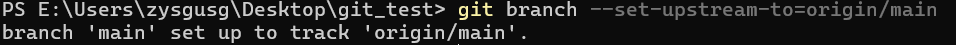
\includegraphics[width=0.8\textwidth]{16.png} 
    \caption{git branch --set-upstream-to=<remote>/<remote branch>}
\end{figure}
\begin{figure}[htbp]
    \centering
    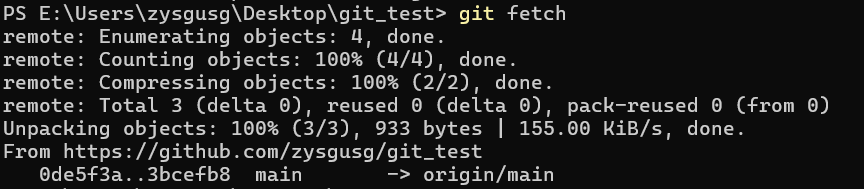
\includegraphics[width=0.8\textwidth]{17.png} 
    \caption{git fetch}
\end{figure}
\begin{figure}[htbp]
    \centering
    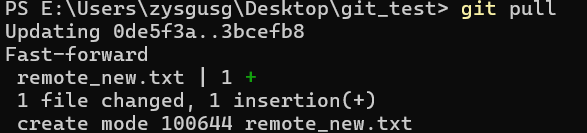
\includegraphics[width=0.8\textwidth]{18.png} 
    \caption{git pull}
\end{figure}
\begin{figure}[htbp]
    \centering
    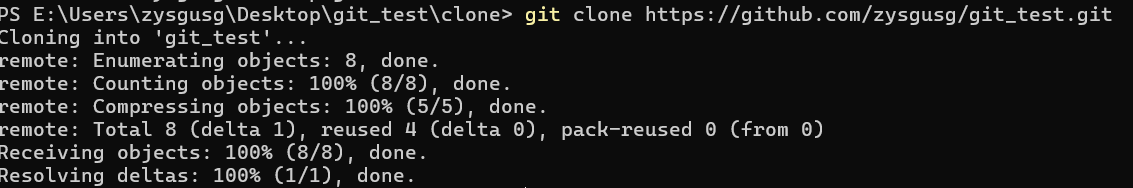
\includegraphics[width=0.8\textwidth]{19.png} 
    \caption{git clone}
\end{figure}
\begin{figure}[htbp]
    \centering
    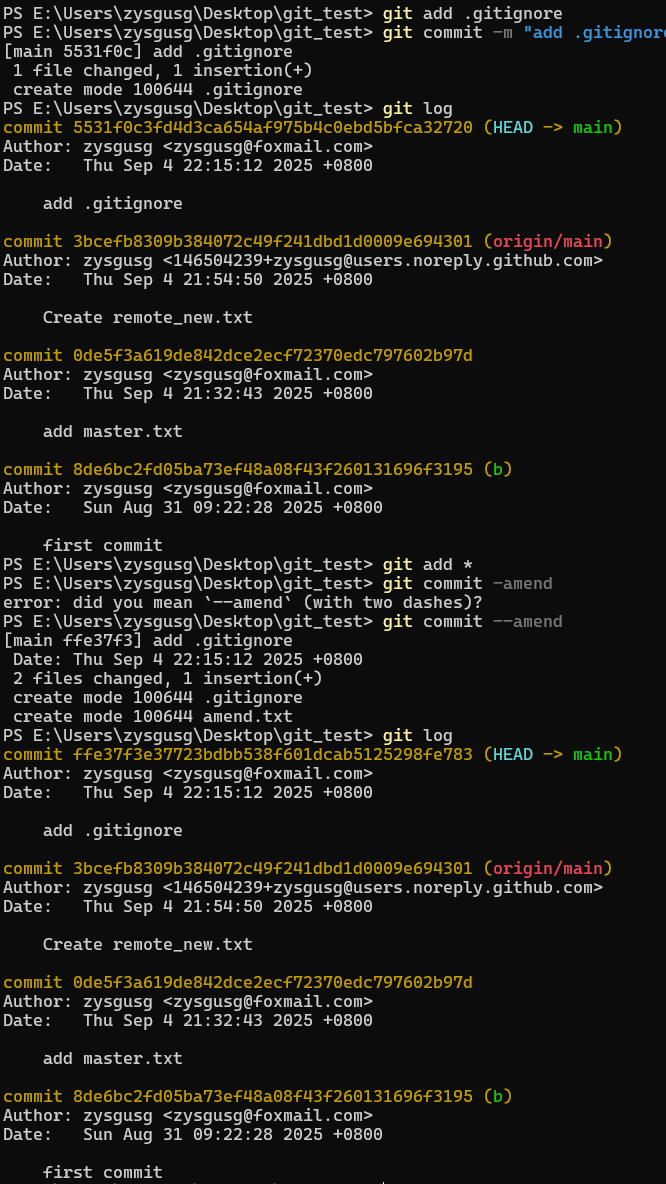
\includegraphics[width=0.8\textwidth]{20.png} 
    \caption{git commit --amend}
\end{figure}
\begin{figure}[htbp]
    \centering
    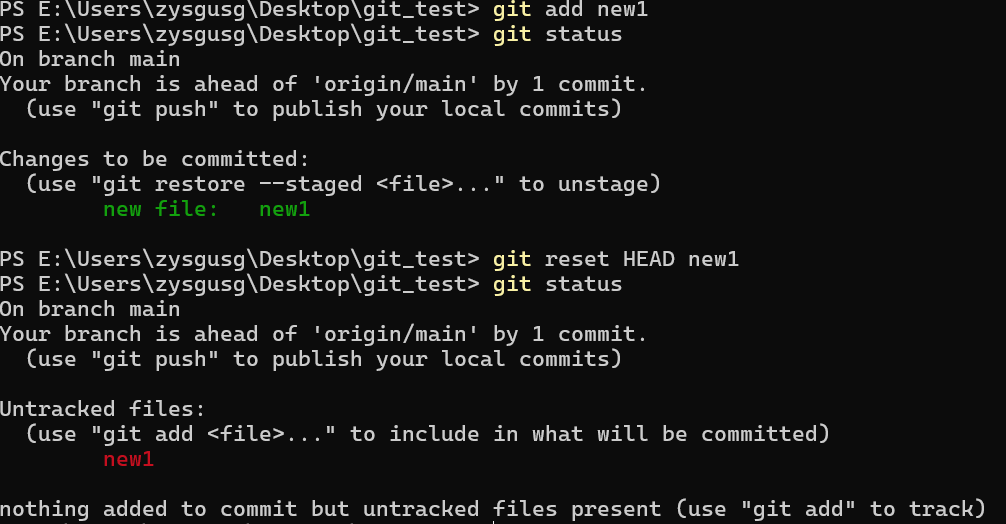
\includegraphics[width=0.8\textwidth]{21.png} 
    \caption{git reset HEAD <file>}
\end{figure}
\begin{figure}[htbp]
    \centering
    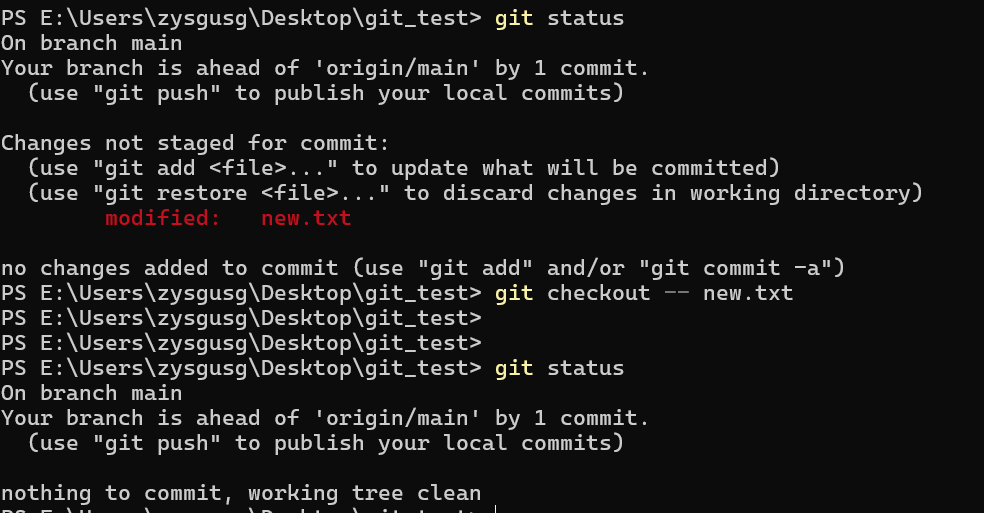
\includegraphics[width=0.8\textwidth]{22.png} 
    \caption{git checkout -- <file>}
\end{figure}

\FloatBarrier %防止图片乱跑
% --- 心得体会 ---
\section{心得体会}
\begin{itemize}
    \item \textbf 通过本次实验,我学到了版本控制相关的知识,加深了对git命令及其实现机制的理解。

\end{itemize}


\end{document}
